\documentclass{article}
\usepackage{graphicx}
\usepackage{wrapfig}
\usepackage{subcaption}
\usepackage[margin=1in]{geometry}
\usepackage{amsmath} % or simply amstext
\usepackage{amssymb}
\usepackage{siunitx}
\usepackage{booktabs}
\usepackage[export]{adjustbox}
\newcommand{\angstrom}{\textup{\AA}}
\newcommand{\colormap}{jet}  % colorbar to use
\usepackage{cleveref}
\usepackage{booktabs}
\usepackage{gensymb}
\usepackage{float}

\title{Using Stochastic Modeling to Predict Long Timescale Transport Behavior of Solutes in an H\textsubscript{II} Phase Lyotropic Liquid Crystal Membrane}
\author{Benjamin J. Coscia \and Michael R. Shirts} 

\begin{document}

  \graphicspath{{./figures/}}
  \maketitle

  \section{Introduction}
  %BJC: obviously this section will get beefed up
  We need highly selective membranes in order to perform efficient separations.

  \noindent Amphiphilic molecules are capable of self-assembling into ordered nanostructures.

  Lytropic liquid crystals are a class of amphiphilic molecules that can be cross-linked
  into mechanically strong membranes.
  \begin{itemize}
  	\item H\textsubscript{II} phase lyotropic liquid crystals have densely packed, uniform
	sized pores and have the potential to disrupt conventional membrane separation
	techniques by being selective based not only on size and charge, but on chemical
	functionality as well.
	\item Q\textsubscript{I} phase LLCs consist of a tortuous network of 3D interconnected
	pores. They are easier to make.
  \end{itemize}

  We can only learn so much from experiment. MD can give us mechanistic insights with
  atomistic resolution so that we can intelligently design new membranes for 
  solute-specific separations.

  In our previous work, we studied the transport of 20 small polar molecules
  in an H\textsubscript{II} phase LLC membrane.
  \begin{itemize}
    \item In general, we observed subdiffusive transport behavior characterized 
    by intermittent hops separated by periods of entrapment.
    \item We identified three mechanisms responsible for the solute trapping behavior:
    entanglement among monomer tails, hydrogen bonding with monomer head groups, and
    association with sodium counter ions.
  \end{itemize}

  % BJC: I've been trying to understand the following justification a bit more. Does it
  % rely on the MSD becoming linear so we can get experimentally diffusion constants? Is
  % it just to try and reduce uncertainty in our MSD predictions? What can we learn from
  % long stochastic simulations that we can't learn from the shorter simulations.
  % BJC: To me the value in this is gaining a deeper mechanistic understanding by 
  % putting things in terms of easily interpreted equations.
  % BJC: Maybe it's just a combination of both.
  Unfortunately, the timescales that we can simulate with MD are insufficient to be
  able to make well-converged predictions of macroscopic transport properties 
  traditionally used to characterize membranes in the lab.

  One can draw from a number of scientific field to model transport behavior as a
  stochastic process.
  \begin{itemize}
    \item In the simulation literature, most start with mean squared displacement (MSD)
    \item Due to the time scales most people simulate, the MSD does not give a complete
    picture of what happens long-term.
    \item Markov state models are popular with researchers of proteins which have 
    many dynamical states occurring over multiple time scales.
    \item The anomalous diffusion literature 
    \item The financial literature studies a wide range of time series behavior which 
    may be particularly useful for describing short time scale dynamics.
  \end{itemize}

  % brief (1 paragraph) review of techniques for predicting long time scale behavior
  The are numerous ways one can approach modeling transport behavior, withing varying
  levels of complexity.
  \begin{itemize}
    \item Most 

    \item Mean first passage time?

    \item Hidden markov models are useful for when states are known but one cannot
  \end{itemize}
  % Ornstein-Uhlenbeck (Gaussian + non-Gaussian)
  
  Talk about finance, single particle tracking and other places this type of analysis
  are used. Use word ubiquitous

  In this work, we explore three approaches to model the long timescale behavior
  of the four solutes fasted moving solutes studied in our previous work.
  \begin{itemize}
    \item Specifically, we study methanol, urea, ethylene glycol and acetic acid
  	\item Our first approach is based on the anomalous diffusion literature.
  	\item The second approach uses Markov state models (MSMs) 
  	\item The third uses an infinite hidden Markov model (iHMM), an unsupervised machine
  	learning algorithm which groups solute behavior into different dynamical states.
  	% BJC: somewhere emphasize that this last approach is powerful since it doesn't 
  	% require anything different in systems with more complex geometries (i.e. QI)
  \end{itemize}

  \section{Methods}
    
  We ran all MD simulations and energy minimizations using GROMACS 2018. We
  performed all post-simulation trajectory using python scripts which are available
  online at \texttt{https://github.com/shirtsgroup/LLC\_Membranes}.

  \subsection{Molecular Dynamics Simulations}

  We studied transport of solutes in the H\textsubscript{II} phase using an
  atomistic molecular model of four pores in a monoclinic unit cell with 
  10 \% water by weight. 
  \begin{itemize}
    \item Approximately one third of the water molecules occupy the tail region 
    with the rest near the pore center.
    \item We chose to study the 10 wt \% water system because solutes move 
    significantly faster than in the 5 wt \% system studied previously.
    \item Appropriate stochastic modeling requires that solutes explore 
    as much structural space as possible.  %BJC: better term than structural space?
  \end{itemize}
  
  We chose to study a subset of 4 of the fastest moving solutes from our previous
  work: methanol, acetic acid, urea and ethylene glycol.
  \begin{itemize} 
    \item In addition to exploring membrane structural space the most, these solutes
    have a relatively diverse set of chemical functionality.   
    \item For each solute we created a separate system and to each system we
    added 6 solutes per pore for a total of 24 solutes.
    \item This number of solutes per pore provides a balance of a low 
    degree of interaction between solutes and sufficient amount of data from
    which to generate statistics on the time scales which we simulate.
    \item Further details on the setup and equilibration of these systems can
    be found in our previous work.\cite{coscia_chemically_2019}
  \end{itemize}
  
  We extended the 1 $\mu$s simulations of our previous work to 5 $\mu$s in order
  to collect ample data.
  \begin{itemize}
    \item We simulated the system with a time step of 2 fs at a pressure of 1 bar
    and 300 K controlled by the Parinello-Rahman barostat and the v-rescale thermostat
    respectively.
  \end{itemize}
  
  \subsection{Markov State Models}\label{method:MSMs}  % BJC: this section first in hopes that sfbm works better
  
  A Markov state model decomposes a time series into a set of discrete states
  with transitions between states defined by a transition probability matrix, T,
  which describes the conditional probability of jumping to a specific 
  state given the previously observed state.~\cite{pande_everything_2010,wehmeyer_introduction_2018}
  \begin{itemize}
    \item In the context of molecular simulations, MSMs are frequently used
    to study systems with slow dynamics, such as protein folding.~\cite{snow_how_2005,chodera_automatic_2007}
    \item Researchers typically aim to come up with a low dimensional 
    representation of the system based on features which preserve the process
    kinetics. This facilitates the identification of discrete states from
    which T is generated.
    \item Software packages such as MSMbuilder~\cite{beauchamp_msmbuilder2:_2011}
    and pyEMMA~\cite{scherer_pyemma_2015} provide work flows capable 
    of featurization and dimensional reduction.
  \end{itemize}
  
  In this work, we define a total of 8 discrete states based on the 3 trapping
  mechanisms observed in our previous work. 
  \begin{itemize}
  	\item Therefore, there is no need to subject our trajectories to any reduction
  	in dimensionality. 
  	%BJC: not sure the best way to lay these out
  	\item The states we've chosen include all combinations of trapping mechanisms 
  	in the pore and out of the pore:
  	\begin{enumerate}
  	  \item Trapped in tails
  	  \item Trapped in tails and hydrogen bonding
  	  \item Trapped in tails and associated with sodium
  	  \item Trapped in tails, hydrogen bonding and associated
  	  \item In pores
  	  \item In pores and hydrogen bonding
  	  \item In pores and associated with sodium
  	  \item In pores, hydrogen bonding and associated
  	\end{enumerate}
  	\item These choices assume that there are no significant kinetic effects resulting
  	from solute conformational changes or pore size fluctuations, an assumption 
  	that may be relaxed in future work.
  	\item However, we will adopt the validation techniques used in the packages
  	mentioned above.  
  \end{itemize}
  
  % BJC: does it make sense to use Dirichlet Process as a conjugate prior for
  % getting error on transition matrix?
  
  \noindent We constructed a state transition probability matrix based on observed solute
  trajectories.
  \begin{itemize}
    \item Using methods described in our previous work, we determined 	
    which, if any, trapping mechanisms affected the solute at each time step, and
    assigned the observation to a specific state according to the definitions 
    above.~\cite{coscia_chemically_2019}
    \item Based on the current and previous state observation, we incremented the
    appropriate entry of an $n x n$ count matrix by 1, where $n$ is the number of states.
    \item For example, if we observed state 1 followed by a transition to state 3,
    we increment the $(1, 3)$ entry of the count matrix by 1.
    \item We generate the transition probability matrix from the count matrix by 
    normalizing the entries in each row so that they summed to unity.
  \end{itemize}
  
  \noindent We recorded the $z$-direction displacement at each time step in order to construct
  individual emission distributions for each state and transition between states.
  \begin{itemize}
    \item While the dynamics of the states themselves are important, the 
    majority of observations involve transitions between states, so properly modeling
    the transition dynamics is even more important.
    %BJC: some of the transitions are pretty rare, so those emission distributions might be less reliable
    \item The shape of the distributions are symmetric and heavy-tailed. 
  \end{itemize}
  
  \noindent We modeled the emission distributions as L\'evy stable distributions.  % cauchy is a case of a Levy stable distribution. The tails are too heavy though.
  \begin{itemize}
    \item For independent and identically distributed (iid) random variables, the 
    generalized central limit theorem guarantees convergence of the associated 
    probability distribution function (PDF) to a L\'evy stable PDF. \cite{klages_anomalous_2008}
    % BJC: ``For sums of independent, iid random variables with proper normalization to the
%    sample size, the generalized central limit theorem guarantees the convergence of
%    the associated PDF to a L\'evy stable PDF even though the variance of these random
%    variables diverges." \cite{klages_anomalous_2008}  % BJC: reword
    \item The characteristic equation describing the Fourier transform of a L\'evy 
    stable PDF is given below:
    \begin{equation}
    p_{\alpha, \beta}(k;\mu,\sigma) = exp\left[i\mu k - \sigma^{\alpha}|k|^{\alpha}\left(1 - i\beta\frac{k}{|k|}\omega(k, \alpha)\right)\right]
    \end{equation}
    \item Where $\omega$ is defined with something that is complicated to format and can be 
    added later if I keep these formulas in. % https://tex.stackexchange.com/questions/32140/how-to-write-a-function-piecewise-with-bracket-outside
    \item $\alpha$ is the index of stability or L\'evy index, $\beta$ is the skewness 
    parameter, $\mu$ is the shift parameter and $\sigma$ is a scale parameter.
    \item The most familiar case, and 1 of 3 that can be expressed in terms of elementary
    functions, is the Gaussian PDF ($\alpha$ = 2).
    \item The more general family of L\'evy stable distributions allows
    greater flexibility in defining the observed emission distribution PDFs.
    \item In the case that the empirical emission distributions are iid, sequential draws
    from a L\'evy stable PDF defines a L\'evy process. 
    \item We can relax the iid assumption and maintain the flexibility of L\'evy stable 
    probability distributions if we instead consider the dynamics to be governed by a
    non-Gaussian Ornstein-Uhlenbeck (OU) process.\cite{barndorffnielsen_non-gaussian_2001} % BJC: replaces Wiener process with Levy process
    \item OU processes contain temporal dependence but the marginal observation distributions
    are consistent with the underlying stochastic driver.~\cite{taufer_simulation_2009}
    \item We will discuss the implications of each.  
  \end{itemize}
  
  L\'evy stable distributions often have heavy tails and an undefined variance 
  which can give rise to arbitrarily long particle displacements.
  \begin{itemize}
  	\item We do not observe hops longer than x nm in our simulations which 
  	emphasizes that these distributions are only an approximation.
    \item We avoid unrealistic, enormous hops problem by truncating the tails
    of the distribution. %BJC: can add some citations about truncated Levy distributions
    \item Since solutes in our system cannot hop further than the length of our 
    simulation unit cell, we truncate the tails of the distribution at this
    magnitude.
    % BJC: Is this actually the right way to do this? I am looking at unwrapped coordinates,
    % so theoretically a particle can move as far as it wants between frames.
    % BJC: The cut-off choice is pretty important and has a significant effect on MSD. 
    % For example, if I truncate at the unit cell length I reproducably get a final MSD of ~ 66 nm^2 (1000 ns stochastic simulation)
    % If I truncate the tails at double the unit cell length, I get a final MSD of ~107 nm^2
    % The uncertainty also increases (since variance diverges for these distributions)
    % So maybe it makes the most sense to truncate based on largest observed hops.
  \end{itemize}
  
  We simulated realizations of the stochastic process using the probability transition
  matrix and emission distributions.
  \begin{itemize}
    \item For each trajectory simulated, we chose an in initial state randomly from a 
    uniform distribution. %BJC: could construct initial distribution but I'm not sure how reliable that is based on 24 solutes that are started in the pore center. (need to chop off beginning 5 ns or so to get rid of that initial dependence)
    \item We randomly drew subsequent state transitions and corresponding emissions 
    from the rows of the probability transition matrix and the appropriate emission
    distribution respectively.
  \end{itemize}
  
  %BJC: need to add some validation of Markovian behavior and time step choice.  
  
  \subsection{Modeling subdiffusion}\label{method:model_sFBM}

  Solutes in this system exhibit subdiffusive behavior, a type of anomalous diffusion.
  \begin{itemize}
  	\item During an anomalous diffusion process, the mean squared displacement (MSD)
  	does not grow linearly with time, rather it is of the form:
	\begin{equation} 
	\langle x^2(t) \rangle = K_{\alpha}t^\alpha
	\label{eqn:msd_form}
	\end{equation} 
	where $\alpha$ is the anomalous exponent and $K_\alpha$ is the
	generalized diffusion coefficient.
	\item A value of $\alpha < 1$ indicates a subdiffusive process, while values of
	$\alpha = 1$ and $\alpha > 0$ are characteristic of Brownian and superdiffusive
	motion respectively.
  \end{itemize}

  \noindent We analyzed both the ensemble-averaged and time-averaged MSDs
  of the simulated trajectories.
  \begin{itemize}
	\item The ensemble-averaged MSD measures the displacement of a particle from its initial
	position~\cite{meroz_toolbox_2015} and can be written as
	\begin{equation}
	\langle x^2(t) \rangle = \langle x(t) - x(0) \rangle^2
	\label{eqn:ensemble_msd}
	\end{equation}
%	\item The average MSD calculated in this way recovers the form of
%	Equation~\ref{eqn:msd_form}. % time-averaged should recover it too for FBM 
	\item The time-averaged MSD measures the displacement between all possible time lags
	and can be written as
	\begin{equation}
	\overline{x^2(\tau)} = \dfrac{1}{T - \tau}\int_{0}^{T - \tau} (x(t + \tau) - x(t))^2 dt
	\end{equation}
	where $\tau$ is the time lag and T is the length of the
	trajectory~\cite{meroz_toolbox_2015}. 
  \end{itemize}
  
  \noindent Three common mathematical models for modeling anomalous subdiffusion
  processes include continuous time random walks (CTRW), fractional Brownian motion
  (FBM) and random walks on fractals (RWF).\cite{meroz_toolbox_2015}
  \begin{itemize}
    \item FBM is common in crowded, viscoelastic environments where each step comes 
    from a Gaussian distribution but is anti-correlated to its previous 
    step.~\cite{mandelbrot_fractional_1968,jeon_fractional_2010,banks_anomalous_2005}
    \item A CTRW is characterized by a distribution of hop lengths and 
    dwell times, where each each step is characterized by independent random draws from 
    each distribution.\cite{montroll_random_1965,morrin_three_2018}
    \item An RWF is imposed by a system's geometry. Systems with tortuous pathways and dead
    ends cause anti-correlated motion.\cite{meroz_toolbox_2015,neusius_subdiffusion_2008}
    \item The processes described above can happen alone or in combination.  	
  \end{itemize}
  
  % BJC: Should this be in the results? Lots of figures to show in support of the claims below
  \noindent We believe that solutes in the system studied here exhibit subordinated 
  fractional Brownian motion (sFBM) where the parent process is FBM and the 
  leading process is a CTRW. 
  \begin{itemize}
  	\item The ensemble-averaged MSD differs from the time-averaged MSD, which
  	is indicative of non-ergodicity, a trait inherent to CTRWs but not FBM or RWFs.~\cite{thiel_weak_2014}  % BJC: need a figure to show this
  	\item We also observe non-stationary $z$-coordinate traces of each solute's
  	center of mass (COM). %BJC: figure of a z-coordinate trace in main text or in supporting info
  	\item For a pure CTRW, the time-averaged MSD should be linear.
  	~\cite{neusius_subdiffusion_2008,meroz_subdiffusion_2010}
  	\item However, a typical time-averaged solute MSD is sublinear (see supporting
  	information), which suggests that there is another underlying subdiffusive mechanism.
  	\item The hop lengths recorded after each dwell period are anti-correlated (See supporting information)
  	\item Given the viscoelastic nature of the monomers in our system, we believe
  	the hop lengths can be modeled with FBM. 
 	\item For subordinated FBM, it can be shown that
  	\begin{equation}
  	\langle x^2(t) \rangle \simeq t^{\alpha\beta}
  	\end{equation}
  	where $\alpha$ is the anomalous exponent characteristic of the leading CTRW process
  	and $\beta$ is the anomalous exponent characteristic of the parent FBM process. 
  \end{itemize}

  \noindent We can characterize a CTRW process using the parameters which describe its
  dwell time and hop length distribution.  % This is different from the emissions of the markov state model where every single step is used to construct the distribution. 
  \begin{itemize}
	\item We used the \texttt{ruptures} python package in order to identify
	changepoints in solute trajectories.\cite{truong_ruptures:_2018} (See Supporting
	Information for more details on chosen parameters. i.e. type of cost function, 
	cost function penalty tolerance, number of dimensions used)
	\item We used the corresponding hop lengths and dwell times between break points
	to construct empirical distributions.
  \end{itemize}
	
  For solutes in our system, the distribution of hop lengths appears to be
  well-represented by a Gaussian distribution.~\cite{metzler_random_2000,
  metzler_anomalous_2014,neusius_subdiffusion_2009}
  \begin{itemize}
	\item We are most interested in the standard deviation, $\sigma$, of the 
	hop length distribution.
  \end{itemize}
  
  \noindent The distribution of dwell times is expected to fit a power law
  distribution proportional to $t^{-1-\alpha}$.~\cite{meroz_toolbox_2015}
  \begin{itemize}
	\item Because we are limited to taking measurements at discrete values
	dictated by the output frequency of our simulation trajectories, we fit the
	empirical dwell times to a discrete power law distribution whose maximum
	likelihood $\alpha$ parameter we calculated by maximizing the following
	likelihood function: 
        \begin{equation}
	\mathcal{L}(\beta) = -n\text{ln}\zeta(\beta, x_{min}) -
	\beta\sum_{i=1}^{n} \text{ln}~x_i 
	\label{eqn:powerlaw_likelihood}
	\end{equation}
	where $\beta = 1 + \alpha$, $x_i$ are collected dwell time data points,
	$n$ the total number of data points, and $\zeta$ is the Hurwitz zeta function
	where $x_{min}$ is the smallest measured value of
	$x_i$.~\cite{clauset_power-law_2009} 
	\item We obtained distributions of the hop length standard deviations, $\sigma$, and
	$\alpha$ using statistical bootstrapping.\cite{efron_introduction_1994} 
  \end{itemize}
  
  \noindent FBM processes can be described using the Hurst parameter, $H$, where 
  $H = \beta/2$.
  \begin{itemize}
  	\item Brownian motion is recovered for $H = 0.5$
	\item The autocovariance function of hop lengths has the analytical form:~\cite{mandelbrot_fractional_1968}
    \begin{equation}
	\gamma(k) = \dfrac{1}{2}\bigg[|k-1|^{2H} - 2|k|^{2H} + |k+1|^{2H}\bigg]
	\label{eqn:autocovariance}
	\end{equation}
	where $k$ is the number of increments between hops.
	\item We obtained H by performing a least squares fit of Equation~\ref{eqn:autocovariance}
	to the empirically measured autocovariance function.
	\item We used statistical bootstrapping to generate a distribution of $H$ 
	values. %BJC: can provide more detail in supporting or just reference python script
  \end{itemize}
  
  % BJC: Is it worth showing performance of both types of models? one mode versus two mode?
  % Probably worth showing that 1 state fails
  % BJC: also not sure if there is a better word than mode. I stayed away from 'state' since
  % it's used heavily in the MSM section.
  % BJC: I haven't created the 2 mode model yet, but that'll only take a few hours. I'll
  % do that after I get BCC equilibrations running
  In general, we observe different dynamical behavior when solutes move inside the
  pore versus in the tail region.
  \begin{itemize}
    \item This inspired two models of varying complexity.
    \item We created a simple, single mode model with a single $\alpha$, $\sigma$ and $H$
    parameter fit to each solute.
    \item Our second, two mode model assigns a set of parameters to each of 2 modes based
    on the solute's radial location.
    \item Solutes in mode 1 are in the pore region defined as less than 0.75 nm from any
    pore center and all else are in mode 2, the tail region. 
    \item We determined this cut-off and described how we calculated radial 
    distance from the pore center in our previous work~\cite{coscia_chemically_2019}
  \end{itemize}

%  We generated distributions of parameters for the dwell time and hop length
%  distributions using statistical bootstrapping.
%  \begin{itemize}
%	\item For each type of distribution, we randomly selected $n$ data points from the empirical
%	distribution with replacement.
%	\item We repeated the fitting procedure described above for each of 200 bootstrap trials.
%  \end{itemize} 

%  We calculated macroscopic diffusion coefficients by simulating trajectories orders of
%  magnitude longer than our molecular simulations.
  \noindent For each solute, we simulated 10000 5 $\mu$s sFBM trajectories. 
  \begin{itemize}
	\item We constructed trajectories by simulating	sequences of dwell times and correlated 
	hop	lengths generated based on parameters randomly chosen from our bootstrapped parameter
	distributions.
	\item We propagated each trajectory until the total time reached 1 $\mu$s, and truncated
	the last data point so that the total time exactly equaled 5 $\mu$s. 
    \item Valid comparisons are only possible between fixed length sFBM simulations. The
    power law dwell time behavior gives rise to the aging phenomenon, embodied by
    a decrease in MSD with measurement time.~\cite{neusius_subdiffusion_2008,metzler_anomalous_2014}
    \item We reported the MSD after 5 $\mu$s with corresponding 95 \% intervals
% Following probably better suited for supporting information, if included at all
%	\item We randomly sample Gaussian hop lengths using the
%	\texttt{numpy.random.normal} method of the \texttt{numpy} python package.
%	\item We randomly sampled dwell times from a discrete power law
%	distribution based on the recommendations of Clauset et
%	al.~\cite{clauset_power-law_2009}: 
%	\begin{equation}
%	x = \lfloor
%	(x_{min} - \tfrac{1}{2})(1 - r)^{-1/(\alpha - 1)} + \tfrac{1}{2} \rfloor
%	\label{eqn:discrete_powerlaw_draws}
%	\end{equation}
%	where $r$ is randomly drawn from a uniform distribution which we simulated
%	with \texttt{numpy.random.uniform}.
%	\item We found that thermal noise does not significantly influence the MSD and
%	therefore did not add any noise to the simulated trajectories. (See supporting info)
  \end{itemize}

%BJC: probably don't need to explain this in great detail
%  \noindent We fixed the length of each simulated trajectory so that we could compare the total
%  MSD between different solutes without the influence of the ageing phenomenon.
%  \begin{itemize}
%	\item Ageing is defined by the tendency of the average MSD to decrease
%	as the length of trajectories are increased~\cite{metzler_anomalous_2014}.
%	\item The maximum measured dwell time can be no longer than the total length
%	of a simulated trajectory. 
%	\item As measurement time or trajectory length is increased, longer dwell times
%	are incorporated into the calculation, lowering the average MSD. (See supporting
%	info for demonstration)
%	\item We can achieve consistent total MSDs with low uncertainty for
%	simulated trajectories created with a given set of parameters if we fix the
%	trajectory length (as opposed to total number of steps).  
%  \end{itemize}

%  \subsubsection*{Coordination number}

%  We quantified the coordination of solutes with surrounding molecules.
%  \begin{itemize}
%  	\item For each frame, we counted the identities and number of
%  	coordinated molecules to a given solute based on a distance cut-off. 
%	\item We found that this approach is more useful than calculating the
%	3D spherical radial distribution function because it gives detailed
%	frame-by-frame information rather than an average. 
%  \end{itemize}

  \subsection{The Infinite State Hidden Markov Model}\label{method:iHMM}  %BJC: potentially a separate paper
  
  Hidden Markov models (HMMs) are a useful and widely used technique
  for modeling sequences of observations where the probability of the next observation
  in a sequence depends only on a previous unobserved, or hidden, state.~\cite{beal_infinite_2002}
  \begin{itemize}
    \item In the context of our simulations, the observations correspond to 
    the center of mass coordinates of the solutes versus time, and the states
    correspond to the dynamical behavior which give rise to those types
    of observations.
    \item Unfortunately, standard HMMs require the number of hidden states to be known
    a priori.
  \end{itemize}
  
  The infinite-state HMM overcomes this drawback by placing a hierarchical
  Dirichlet process (HDP) prior on the transition probabilities.
  \begin{itemize}
    \item Using some base probability distribution, H, a Dirichlet process 
    (DP) generates distributions over a countably infinite number of 
    probability measures:
    \begin{equation}
      G_0 = \sum_{k=1}^{\infty} \beta_k \delta_{\theta_k} ~~ \theta_k \sim H, \beta \sim GEM(\gamma)
    \end{equation}
    where the $\theta_k$ are values drawn from the base distribution and the
    weights $\beta_k$ come from a stick-breaking process parameterized by the concentration 
    parameter $\gamma$ (equivalently referred to as GEM($\gamma$)). 
    \item The concentration parameter expresses one's confidence in H relative to the posterior 
    and is closely related to the number of data observations.
    \item Each row, $G_j$, of the transition matrix is produced by drawing from a DP specified 
    using the $\beta$ vector as a discrete base distribution and a separate concentration
    parameter, $\alpha$.
    \begin{equation}
      G_j = \sum_{k=1}^{\infty} \pi_{jk} \delta_{\theta_k} ~~ \pi_j \sim DP(\alpha, \beta)
    \end{equation}
    \item This hierarchical specification ensures that the transition probabilities in 
    each row share the same support points \{$\theta_1$, ..., $\theta_k$\}.
  \end{itemize}
   
  \noindent We describe the dynamics of each state using a vector autoregressive (VAR) model. 
  \begin{itemize}
  	\item A VAR process is characterized by a vector of observations in a time series 
  	that are dependent on $r$ previous values of the time series vector, weighted by a
  	coefficient matrix $A_i$ in addition to a white noise term $\mathbf{e}_t$:
  	\begin{equation}
  	\mathbf{y}_t = \sum_{i=1}^r A_i\mathbf{y}_{t-i} + \mathbf{e}_t~~~~\mathbf{e}_t \sim N(0, \Sigma)
  	\end{equation}
  	\item We assumed multivariate Gaussian noise and limited our analysis to an 
  	autoregressive order of $r=1$.
  	\item We used a conjugate matrix-normal inverse-Wishart prior on parameters
  	$A$ and $\Sigma$ in order to analytically draw from the posterior.
  \end{itemize}   
  
  Based on the VAR parameters and matrix of transition probabilities, we calculated
  the most likely sequence of hidden states.
  \begin{itemize}
    \item We repeated this process iteratively until we reached convergence % BJC: need to define convergence criteria
    \item Our python implementation of this process is heavily adapted from the MATLAB code
    of Fox et al.~\cite{fox_sticky_2007} 
    \item We refer the interested reader to much more extensive descriptions of 
    this process and its implementation. 
    ~\cite{beal_infinite_2002,teh_hierarchical_2006,van_gael_beam_2008,fox_nonparametric_2009,fox_bayesian_2010}
  \end{itemize}
  \break
  \section{Results and Discussion}
  
  \subsection{Molecular Dynamics Simulations}\label{section:MD_simulations}
  
  The MSDs for of the solutes calculated from 5 $\mu s$ MD simulation trajectories
  are shown in Figure TBD.
  \begin{itemize}
    \item 2 options for a figure:
    \item 1) 2 panels: 1st panel: bar chart with final MSD value + error bars. 2nd panel: a selected MSD curve
    \item 2) 1 panel. All MSD curves. Overlapping errors might look bad
  \end{itemize}
  
  Solute motion is influenced by the same three trapping mechanisms observed in our
  previous works.
  \begin{itemize}
    \item The extent to which each trapping mechanism influences each solute is
  depicted graphically in Figure TBD.
    \item Same types of figures from transport paper:
    \item Fraction participating in hydrogen bonds, fraction associated, fraction
    in the tails.
    \item Lifetimes of hbonds and sodium associations?
  \end{itemize}
  
  \subsection{Markov State Model Fits}\label{section:msm_results}
  
  The emission distributions are non-Gaussian and heavy-tailed (see Figure~\ref{fig:emissions_MET}).
  \begin{itemize}
    \item The heavy tails of the distribution are a consequence of hopping.
    \item Heavily sampled states fit well to L\'evy stable distributions.
    \item The rarer states have less data, but we still assume L\'evy stable distributions.
  \end{itemize}
  
  % BJC: worth proving these are non-Gaussian? One might argue that they look Gaussian but they are not at all.
  \begin{figure}[!h]
  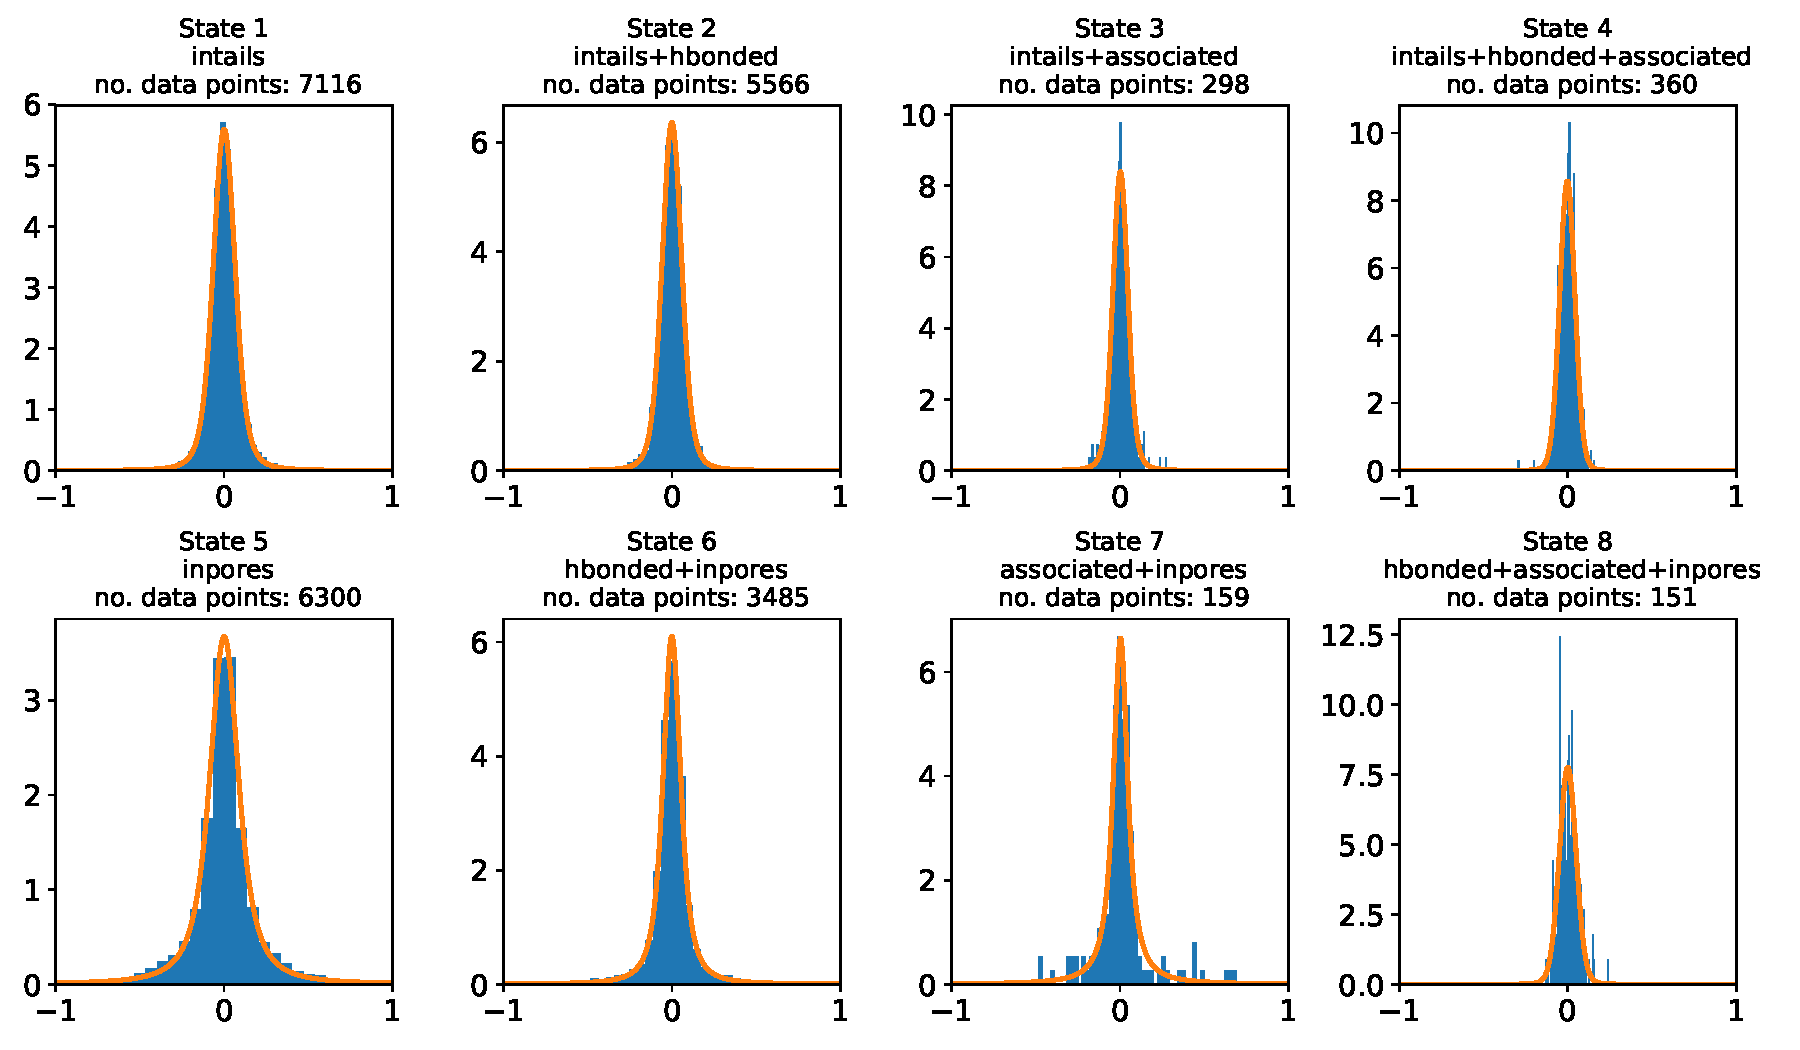
\includegraphics[width=\textwidth]{emissions_MET.pdf}
  \caption{}\label{fig:emissions_MET}
  \end{figure}

  % BJC: need better or more descriptive way of describing stochastic simulations
  % BJC: or could say that whenever we say simulations, we mean stochastic simulations unless it is specified as a molecular dynamics simulation.
  Simulating solute trajectories (see Section~\ref{method:MSMs}) by drawing independent  
  observations from the emission distributions yields near linear MSD curves
  with final values that are far higher than those observed in our molecular simulations.
  \begin{itemize}
	% BJC: right number of solute trajectories to simulate for comparison? More tightens the error bars
    \item In the case of methanol, the final MSD value is about 25x higher than that observed in our
    previous transport study (see Figure~\ref{fig:msd_MET}).
    \item The linear behavior of the MSD curve is not consistent with subdiffusion.
  \end{itemize}

  \begin{figure}[!h]
  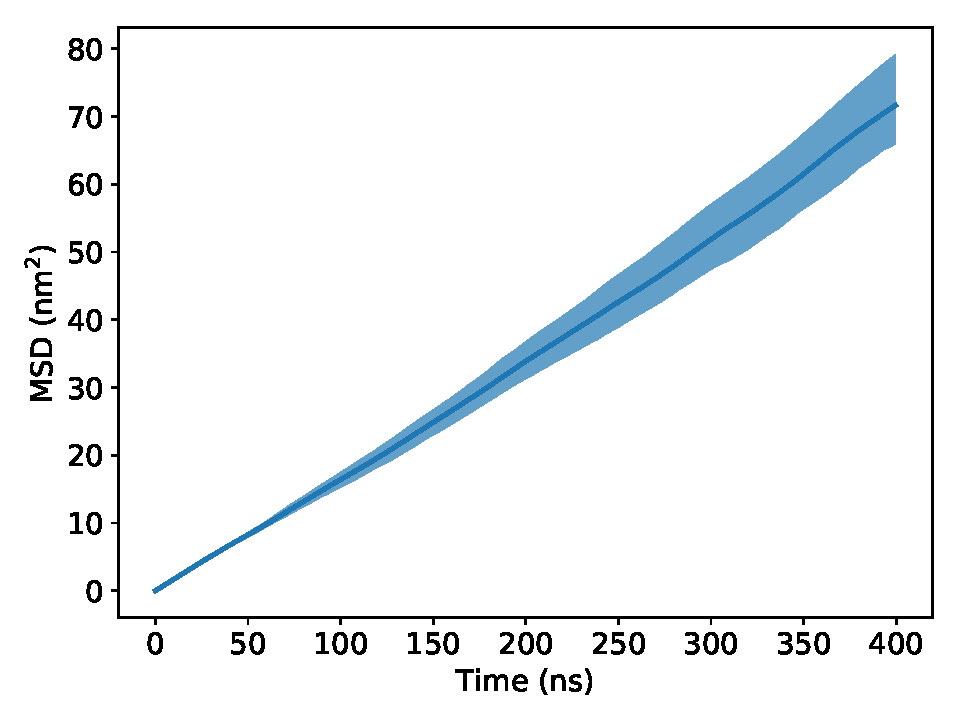
\includegraphics[width=\textwidth]{MET_msd.pdf}
  \caption{}\label{fig:msd_MET}
  \end{figure}
  
  Anti-correlation between hops may be responsible for subdiffusive behavior.
  \begin{itemize}
    \item In general, we observe negative correlation between hops.
    \item A L\'evy driven OU process may be a more appropriate way to model
    the stochastic dynamics of this system since you can incorporate autocorrelation.
    \item Extracting reliable correlation functions is difficult with our data
    due to relatively frequent switching resulting in sets of short disjoint time 
    series describing each state.
    \item Therefore we did not do this and attempted to fit a different model. 
    %BJC: we could add some artificial correlation to test the anti-correlation hypothesis
  \end{itemize}

  \subsection{Subordinated Fractional Brownian Motion Modeling}\label{section:sFBM}
  
  Using the techniques from Section~\ref{section:model_sFBM}, we extracted values 
  of $\sigma$, $\alpha$ and $H$ for each solute for the 1 and 2 mode model 
  (see Table~\ref{table:sfbm_params}).
  \begin{itemize}
    \item In most cases, it is easy to relate $\sigma$, $\alpha$ and $H$ to the
    simulated MSD values presented in Table~\ref{table:simulations}. 
  	\item Higher values of $\sigma$ indicate larger average hop lengths.
  	\item Higher values of $\alpha$ mean that there will be less sampling of 
  	long dwell times.
  	\item Values of $H$ near the Brownian limit of 0.5, indicate a lower degree
  	of anti-correlation.
  	\item All of which contribute to an overall increase in the MSD.
  \end{itemize}
  
  % BJC: worth including single parameter model (i.e. no radial dependence) to 
  % show its shortcomings? Or send to supporting information
  % BJC: obviously still needs 2 mode data
  \begin{table}[h]
  \centering
  \begin{tabular}{cccc}
  \toprule
  System & $\sigma$ ($nm$) & $\alpha$ & $H$ \\
  \midrule
  Methanol & 0.46 & 0.85 & 0.40 \\
  Urea & 0.33 & 0.64 & 0.40 \\
  Ethylene Glycol & 0.35 & 0.64 & 0.36 \\
  Acetic Acid & 0.28 & 0.51 & 0.44 \\
  \bottomrule
  \end{tabular}
  \caption{We calculated values $\sigma$, $\alpha$ and $H$ from MD simulation
  trajectories and then computed the average ensemble-averaged MSD of 10000 
  simulated trajectories.}\label{table:sfbm_params}
  \end{table}

  \noindent We compared the MSD of simulated sFBM trajectories to MD simulated
  MSDs.
  \begin{itemize}
	\item We simulated 10000 sFBM trajectories of the same length as our MD
	simulations, as described in Section~\ref{section:model_sFBM} of the Methods.
	\item The final MSDs of the sFBM trajectories are compared to those 
	calculated directly from MD simulations in Figure~\ref{fig:all_msds}. 
	\item We would like to emphasize that we rely on the MD MSD values in order to
	define trends in the total MSD, while the sFBM trajectories and parameter 
	values allow us to speculate as to the reasons for the observed trends. 
	\item There is a non-negligible amount of error in the calculation of 
	each parameter which prevents us from reliably portraying our sFBM MSDs as
	reduced	uncertainty MD MSDs.
	% BJC: I think it's more the power law tails that increases uncertainty.
  \end{itemize}
  
  The two-mode sFBM model does a better job than the one-mode model at 
  reproducing the MD MSD trends. 
  \begin{itemize}
    \item One-mode model generally undershoots MSDs.
  \end{itemize}

  %BJC: reduce this figure to solutes studied and put 3 bars for each solute: MD MSD, one-mode sfbm MSD, two-mode sfbm MSD
  \begin{figure}
  \centering
  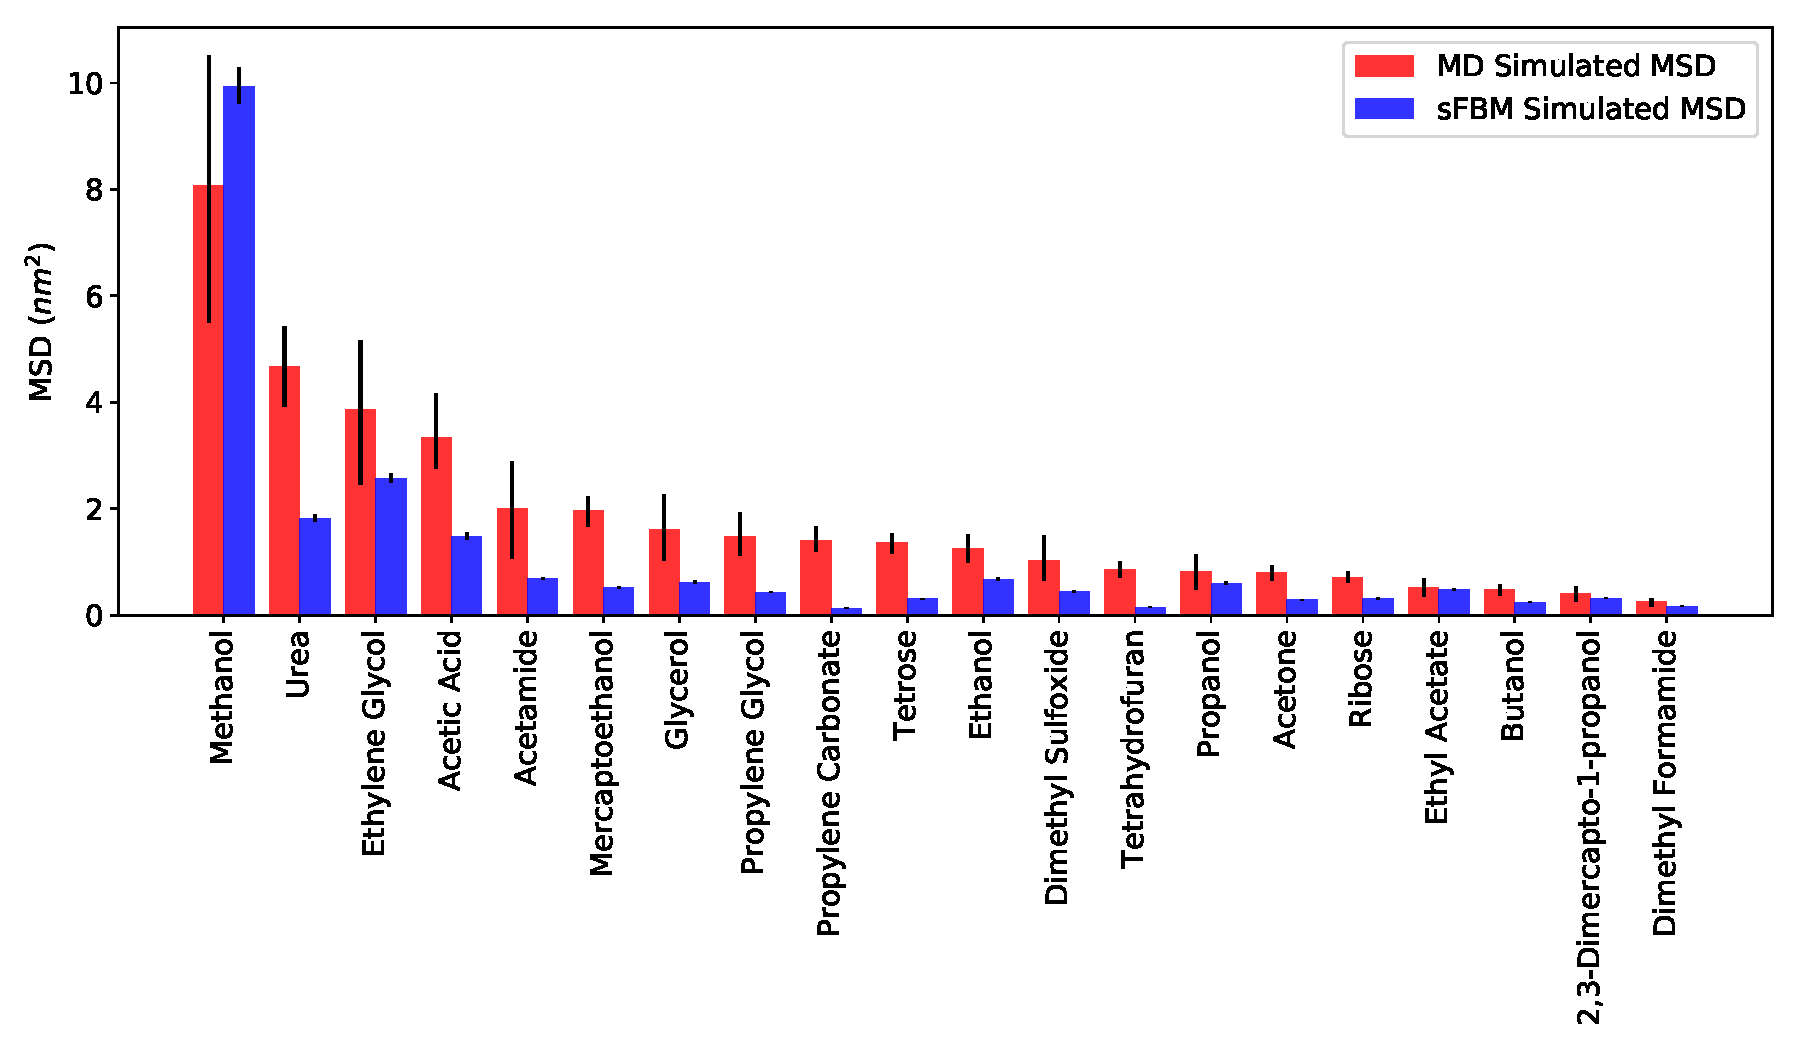
\includegraphics[width=\textwidth]{all_emsds.pdf}
  \caption{}\label{fig:all_msds}
  \end{figure}

  \section{Conclusion}
  
  We have tested two different mathematical frameworks for describing solute
  motion in an H\textsubscript{II} phase LLC membrane.
  \begin{itemize}
    \item Markov state modeling with predefined states gives a nice description
    of transitions between observed states as well as the type of stochastic 
    behavior shown in each state. However, it doesn't accurately portray correlated
    time series behavior leading to overpredicted MSDs.
    \item Subordinated fractional Brownian motion has a nice theoretical foundation
    in the anomalous diffusion literature. A two mode model that describes dynamics
    based on whether a solute is in or out of the pore region leads to MSDs fairly
    consistent with MD simulated trajectories.
  \end{itemize}
 
  \section*{Supporting Information}

  Detailed explanations and expansions upon the results and procedures mentioned in
  the main text are described in the Supporting Information. This information is
  available free of charge via the Internet at http://pubs.acs.org.

  \section*{Acknowledgements}

  Molecular simulations were performed using the Extreme Science and
  Engineering Discovery Environment (XSEDE), which is supported by National
  Science Foundation grant number ACI-1548562. Specifically, it used the Bridges
  system, which is supported by NSF award number ACI-1445606, at the Pittsburgh
  Supercomputing Center (PSC). This work also utilized the RMACC Summit supercomputer,
  which is supported by the National Science Foundation (awards ACI-1532235 and
  ACI-1532236), the University of Colorado Boulder, and Colorado State
  University. The Summit supercomputer is a joint effort of the University of
  Colorado Boulder and Colorado State University.

  \clearpage

  \bibliographystyle{ieeetr}
  \bibliography{stochastic_transport}

  \newpage

  \section*{TOC Graphic}

\end{document}
